\documentclass[11pt]{article}

% Change "review" to "final" to generate the final version.
\usepackage[review]{acl}

% Standard package includes
\usepackage{times}
\usepackage{latexsym}

% For proper rendering and hyphenation of words containing Latin characters
\usepackage[T1]{fontenc}
\usepackage[utf8]{inputenc}
\usepackage{microtype}
\usepackage{inconsolata}

% Additional packages
\usepackage{amsmath,amssymb,amsfonts}
\usepackage{graphicx}
\usepackage{booktabs}
\usepackage{xcolor}
\usepackage{cleveref}

% =============================================================================
% Custom Commands
% =============================================================================
\newcommand{\tocite}{\textcolor{red}{[Add citation]}}
\newcommand{\TODO}[1]{\textcolor{blue}{[TODO: #1]}}

% =============================================================================
% Title and Authors
% =============================================================================
\title{Dissecting Memory in State Space Models}

\author{
    Yuval Ran-Milo \\
    Tel Aviv University \\
    \texttt{yuval@example.com} \\\And
    Shahar Mendel \\
    Tel Aviv University \\
    \texttt{shahar@example.com} \\\And
    Ido Avnir \\
    Tel Aviv University \\
    \texttt{ido@example.com}
}

\begin{document}
\maketitle

% =============================================================================
% Abstract
% =============================================================================
\begin{abstract}
Sub-quadratic models such as Mamba and RWKV compress all past context into a fixed-size recurrent state, raising the question of how effectively they store and retrieve in-context information. We investigate this by probing the internal states of RWKV-7 1.5B on controlled entity-binding tasks and find that: (i) entity-property bindings are concentrated in a small subset of universal memory heads that generalize across semantic domains; (ii) these heads have a direct causal effect on model outputs (iii) probe accuracy far exceeds the model's own retrieval accuracy, revealing a query bottleneck rather than a storage limitation; and (iv) semantically similar context accelerates forgetting. These findings suggest that improving sub-quadratic models may benefit more from better query mechanisms than from increased state capacity.
\end{abstract}

% =============================================================================
% Introduction
% =============================================================================
\section{Introduction}
\label{sec:introduction}

Transformer-based language models have achieved remarkable success across a wide range of tasks \cite{brown2020fewshot}, but their self-attention mechanism scales quadratically with sequence length, making long-context inference expensive \cite{vaswani2017attention}. This has motivated a growing family of sub-quadratic architectures, including state space models (SSMs) such as Mamba \cite{gu2023mamba}, RWKV \cite{peng2023rwkv}, and GLA \cite{yang2023gla}, which achieve linear-time inference by compressing all past context into a fixed-size recurrent state. These models have become competitive with transformers at similar scales \cite{gu2023mamba,peng2025rwkv7}, yet a fundamental tension remains: the state has finite capacity, so it cannot preserve all information from an arbitrarily long context. Something must be forgotten.

This raises a natural question: when information is provided entirely in context, how much of it actually ends up in the state, and how well can the model retrieve it? Moreover, beyond performance, how does this process work mechanistically: where in the model is memory stored, how is it organized, and what determines whether a piece of information can be recovered? Prior work has studied the recall and state-tracking abilities of SSMs through behavioral benchmarks \cite{jelassi2024repeat,fu2022h3,grazzi2024statetracking}, but relatively little is known about what is happening inside the state itself. Is poor recall due to information never being stored, or due to the model failing to extract what is already there?

We address this question by probing the internal states of RWKV-7 1.5B on controlled entity-binding tasks, where each input prompt contains a set of entity-property associations (e.g., ``Lady Gaga's favorite color is red'') that vary randomly across samples. Thanks to the fact that these associations are never seen during pretraining, any successful retrieval must rely on in-context memory. We design probes that respect the architecture's native query mechanism: SSMs produce outputs by right-multiplying the state with a query vector, so we train probes that query the state in the same way. To validate that the heads identified by probing are genuinely involved in memory, we complement our probing analysis with counterfactual patching experiments that test for causal influence on the model's outputs.

In this work we ask: \emph{can we leverage the internal states of SSMs to understand how they store and retrieve in-context information, and where this process breaks down?}

Our main findings are as follows. First, probing reveals that entity-property bindings are reliably encoded in a small subset of heads, with the best head reaching 96.3\% accuracy, and that querying from the right (the natural direction) substantially outperforms querying from the left. Second, counterfactual patching confirms that replacing just 4 out of 768 heads is enough to change the model's answer, while replacing the same number of random heads has almost no effect. Third, the same small set of heads is important across semantically distinct domains, suggesting they function as universal memory heads. Fourth, probe accuracy far exceeds the model's own retrieval accuracy, indicating that the bottleneck lies in querying the state rather than in storing information. Finally, we show that semantically similar context accelerates forgetting, consistent with subspace interference in the state matrix.

% =============================================================================
% Related Work
% =============================================================================
\section{Related Work}
\label{sec:related_work}

\paragraph{Memory in Transformers.}
Transformers implement in-context memory primarily through self-attention, where
each token can retrieve information from earlier positions by computing
content-dependent weights over key--value pairs \cite{vaswani2017attention}.
This mechanism is often viewed as a form of differentiable, content-addressable
memory: rather than compressing the past into a single recurrent state, the
model maintains access to a growing set of past representations, enabling
flexible retrieval and composition over the entire context window. A large body
of work has therefore focused on extending the effective context length or
augmenting the model with additional memory beyond the fixed window. Notable
approaches include recurrence across segments (Transformer-XL), which reuses
previous hidden states to model dependencies beyond a fixed-length context
\cite{dai2019transformerxl}, compressing older memories to preserve long-range
information under a bounded compute budget \cite{rae2019compressive}, and
retrieval-augmented language modeling, which explicitly consults an external
datastore during generation \cite{borgeaud2022retro}. These methods primarily
target \emph{memory availability} (how much information can be brought into the
computation) and \emph{access} (how that information can be retrieved when
needed).

%\paragraph{Sub-quadratic attention and memory.}
%Since standard attention scales quadratically with sequence length, efficient
%Transformer variants aim to preserve attention-like retrieval while reducing
%time and/or memory. Dense approximations typically exploit structure in the
%attention matrix, such as low-rank projections (Linformer)
%\cite{wang2020linformer} or kernel-based approximations with random features
%(Performer) \cite{choromanski2021performer}. Other approaches use approximate
%nearest-neighbor search or hashing to restrict attention computation (Reformer)
%\cite{kitaev2020reformer}. These models are frequently evaluated on long-context
%benchmarks designed to stress memory and long-range dependency modeling, such as
%Long Range Arena (LRA) \cite{tay2020lra}. A recurring theme across this
%literature is that the \emph{form} of the attention approximation matters:
%changing the mechanism used for retrieval (e.g., low-rank vs.\ kernel vs.\
%sparsity) can alter which long-range dependencies remain accessible, thereby
%affecting apparent memory performance even when the nominal context length is
%unchanged.

\paragraph{Attention-free sub-quadratic sequence models.}
A complementary line of work achieves sub-quadratic (often linear-time)
inference by replacing attention with recurrent or convolutional updates that
compress the past into a fixed-size state. State space models (SSMs) provide a
particularly unified view: they maintain an internal state updated online and
produce outputs via a readout from that state. Foundational work on HiPPO
introduced principled mechanisms for online compression of history via
projections \cite{gu2020hippo}. Building on these ideas, structured
parameterizations such as S4 made SSMs computationally practical and competitive
on long-range tasks \cite{gu2021s4}, and subsequent simplifications like DSS
showed that diagonal state parameterizations can retain much of S4's
effectiveness \cite{gupta2022dss}. Modern language-model-scale architectures
(e.g., selective SSMs and gated linear attention variants) can often be
interpreted as instances of this broader paradigm: the model stores information
in a recurrent state and must \emph{query} or \emph{read} from it during
generation. This raises a distinct memory question from the Transformer setting:
when the past is compressed into a fixed-size state, the limiting factor may be
less about what can be stored in principle and more about which stored
information is practically retrievable given the model's readout mechanism.

\paragraph{Entity binding as an in-context memory primitive.}
Entity--attribute binding tasks probe a core capability underlying factual
recall and multi-entity reasoning: given a context describing several entities
and their properties, the model must correctly bind each property to its
corresponding entity at query time. Recent work has used controlled settings to
study how binding is represented internally; for example, Feng and Steinhardt
identify a ``binding ID'' mechanism and use causal interventions to argue that
models attach binding-related vectors to entity and attribute positions
\cite{feng2024binding}. Such findings motivate synthetic entity-binding
evaluations as a targeted lens on in-context memory that avoids confounds from
pretraining knowledge. Our entity-binding datasets are in this spirit, but we
focus on sub-quadratic models whose memory is mediated by a recurrent state:
this shifts the emphasis from \emph{Can tokens attend to the right binding} to
\emph{which bindings are present in the compressed state and how the model
queries them}. In particular, by comparing what can be decoded from the state to
what the model actually retrieves during generation, we align entity binding
with a concrete hypothesis about the failure mode in sub-quadratic
architectures: a potential mismatch between \emph{stored} information and the
model's \emph{query} mechanism.

\paragraph{Interpretability tools for studying memory mechanisms.}
Our work sits within mechanistic interpretability, which aims to localize and
characterize internal computations responsible for model behavior. Probing
methods train auxiliary predictors to decode information from hidden
activations; recent 'lens' techniques decode intermediate representations into
output distributions, providing a token-level view of how predictions evolve
across depth \cite{belrose2023tunedlens}. Beyond correlational probes, causal
interventions are commonly used to establish necessity and sufficiency of
components. Meng et al.\ develop causal tracing interventions to localize
computations supporting factual recall and show that specific mechanisms can be
edited (ROME) \cite{meng2022rome}. Activation patching has become a standard causal tool for circuit-level analysis, and
recent work systematizes methodological choices and metrics for patching-based
localization \cite{zhang2023patching}. Broader frameworks for circuit-based
reasoning about Transformers provide a language for decomposing computations
into interpretable parts \cite{elhage2021framework}. We adopt these
interpretability principles in the sub-quadratic setting by (i) designing probes
that mirror the architecture's native readout direction and (ii) using
counterfactual patching on internal state representations to test whether
probe-identified components have a causal effect on retrieval.


% =============================================================================
% State Space Models
% =============================================================================
\section{State Space Models}
\label{sec:ssm}

Many state-of-the-art sub-quadratic architectures, including Mamba \cite{gu2023mamba}, RWKV \cite{peng2023rwkv}, GLA \cite{yang2023gla}, and Deltanet \cite{yang2024deltanet}, can be unified under the framework of \emph{state space models} (SSMs); see \cref{sec:ssm_examples} for concrete examples. Despite their architectural differences, all of these models can be written in the following generic form.

The model maintains an internal state $S_t \in \mathbb{R}^{d \times d}$ that is updated at each time step based on the previous state and the current input $x_t \in \mathbb{R}^{d}$:
\begin{align}
    S_t &= f(S_{t-1}) + g(x_t), \label{eq:state_update} \\
    o_t &= S_t \, q(x_t), \label{eq:state_query}
\end{align}
where $f$ is a decay or transformation function applied to the previous state, $g(x_t)$ is some function of the current input (independent of other timesteps), and $o_t \in \mathbb{R}^{d}$ is the output. The output is produced by \emph{querying} the state via right-multiplication with a query vector $q(x_t) \in \mathbb{R}^{d}$ derived from the current input.

Unlike transformers, whose attention mechanism incurs $O(L^2)$ computational cost with respect to sequence length $L$, SSM-based models enable inference in $O(L)$ time. This efficiency comes from compressing all past information into a fixed-size state $S_t \in \mathbb{R}^{d \times d}$, which is updated incrementally rather than recomputed from scratch.

This raises a fundamental question: given the finite capacity of the state, \emph{how does the model store and retrieve in-context information?}

\subsection{Examples}
\label{sec:ssm_examples}

To illustrate the generality of this framework, we show how two popular architectures fit the SSM formulation.

\paragraph{Gated Linear Attention \cite{yang2023gla}.}
In GLA, the state update and query take the form:
\begin{equation}
    S_t = S_{t-1} \odot (1 \alpha_t^\top) + v_t k_t^\top, \; o_t = S_t \, q_t,
    \label{eq:gla}
\end{equation}
where $\odot$ denotes element-wise multiplication, and $\alpha_t, v_t, k_t, q_t \in \mathbb{R}^{d}$ are learned projections of the input.

\paragraph{Mamba-2 \cite{dao2024ssmduality}.}
In Mamba-2, the formulation is:
\begin{equation}
    S_t = \gamma_t S_{t-1} + v_t k_t^\top, \; o_t = S_t \, q_t,
    \label{eq:mamba}
\end{equation}
where $\gamma_t \in \mathbb{R}$ is a learned scalar decay factor.

Both architectures share the key property that the output is produced by querying the state from the right.

% =============================================================================
% Methodology
% =============================================================================
\section{Methodology}
\label{sec:methodology}

\subsection{Entity-Binding Datasets}
\label{sec:datasets}

We construct \emph{in-context} entity-binding datasets to study how SSMs store and retrieve factual associations. Each dataset follows a generic structure: samples consist of $N_e$ statements of the form ``\texttt{<entity> <relation> <property>}'', where each entity is associated with one of $C$ possible property values.

These associations are provided entirely within the input prompt (not learned during pretraining) and vary randomly across samples. One designated \emph{target entity} appears in all samples, but its associated property changes. The order of entities is randomized, and the target entity appears at a random position. This ensures that any successful retrieval must rely on in-context memory rather than memorized facts. We generate 10{,}000 prompts per dataset for probing experiments and 50 sample pairs for counterfactual patching. See \cref{fig:dataset_examples} for examples.

\begin{figure}[t]
\centering
\small
\fbox{\parbox{0.9\columnwidth}{
\textbf{Favorite Color} ($N_e=30$, $C=10$)\\[2pt]
\textit{Relation:} ``X's favorite color is Y.''\\[4pt]
\texttt{Lady Gaga's favorite color is red.}\\
\texttt{Beyonc\'{e}'s favorite color is green.}\\
\texttt{...}
}}

\vspace{0.5em}

\fbox{\parbox{0.9\columnwidth}{
\textbf{Lives in City} ($N_e=30$, $C=10$)\\[2pt]
\textit{Relation:} ``X lives in Y.''\\[4pt]
\texttt{The shark lives in France.}\\
\texttt{The dog lives in Italy.}\\
\texttt{...}
}}
\caption{Examples from our entity-binding datasets. Each sample contains $N_e$ entity-property pairs with one target entity whose property varies across samples.}
\label{fig:dataset_examples}
\end{figure}

\subsection{Probing State Representations}
\label{sec:probing}

Recall from \cref{eq:state_query} that SSMs produce outputs by querying the state via right-multiplication: $o_t = S_t \, q(x_t)$. This suggests a natural way to probe whether entity-property bindings are stored in the state: we can train a probe that mimics this query mechanism.

For each internal state $S_t \in \mathbb{R}^{d \times d}$ (indexed by layer $\ell$ and head $h$), we extract the state at the \emph{final token position} of the input sequence. We then train a probe with two learned components: (i) a \textbf{query component} $q_{\text{probe}} \in \mathbb{R}^{d}$ that queries the state from the right, producing $S_t \, q_{\text{probe}} \in \mathbb{R}^{d}$; and (ii) a \textbf{classifier component} $W_{\text{cls}} \in \mathbb{R}^{C \times d}$ that maps the queried vector to $C$ class logits.

The full probe is:
\begin{equation}
    \text{probe}(S_t) = W_{\text{cls}} \, S_t \, q_{\text{probe}} \in \mathbb{R}^{C}.
    \label{eq:probe}
\end{equation}

We call this the \textit{natural probe} because it mirrors the model's native state-querying mechanism: the state is multiplied by a vector \emph{from the right}, just as in \cref{eq:state_query}.

\begin{figure}[t]
    \centering
    \small
    \fbox{\parbox{0.9\columnwidth}{
    \texttt{Given the following context, let's}\\
    \texttt{answer the question below.}\\[4pt]
    \texttt{Context:}\\
    \texttt{Lady Gaga's favorite color is red.}\\
    \texttt{Beyonc\'{e}'s favorite color is green. ...}\\[4pt]
    \texttt{Question: What is Lady Gaga's}\\
    \texttt{favorite color?}\\[4pt]
    \texttt{Answer: Lady Gaga's favorite color is}
    }}
    \caption{Prompt template for evaluating model retrieval. The model must generate the correct property (e.g., ``red'') as the next token.}
    \label{fig:prompt_template}
\end{figure}

To validate that this structure is important, we also train a \textit{non-natural probe} that queries from the opposite direction:
\begin{equation}
    \text{probe}_{\textit{non-nat}}(S_t) = (q_{\text{probe}}^\top S_t) W_{\text{cls}} \in \mathbb{R}^{C},
    \label{eq:probe_wrong}
\end{equation}
where $q_{\text{probe}} \in \mathbb{R}^{d}$ is applied from the left, and $W_{\text{cls}} \in \mathbb{R}^{d \times C}$ projects to class logits. If memory is encoded consistently with the model's query mechanism, the \textit{natural probe} should significantly outperform the \textit{non-natural probe}; we verify this in \cref{sec:probing_ablation}.

\subsection{Training Details}
\label{sec:training_details}

We train each probe with a 70/30 train/validation split, up to 20{,}000 epochs with early stopping (patience of 20 epochs), a batch size of 1{,}000, and a learning rate of $10^{-3}$ using the Adam optimizer.

\subsection{Evaluating Model Retrieval}
\label{sec:model_retrieval}

To compare probe accuracy with the model's own retrieval ability, we construct a question-answering prompt that queries the model for the target entity's property. \cref{fig:prompt_template} shows an example for the Favorite Color dataset.



We measure top-1 accuracy: the model must generate the correct property label as its next token, where we only consider tokens corresponding to valid property values from the dataset (e.g., the $C=10$ colors).

\subsection{Causal Intervention}
\label{sec:causal}

To establish that the heads identified by probing have a \emph{causal} effect on model behavior, we perform counterfactual patching experiments using the prompt structure from \cref{sec:model_retrieval}.

The procedure is as follows: (i) generate two prompts $A$ and $B$ that differ only in the target entity's property (e.g., ``Lady Gaga's favorite color is red'' vs. ``Lady Gaga's favorite color is blue''); (ii) run both prompts through the model, collecting states after processing the context; (iii) for prompt $A$, replace the states of a \emph{subset} of heads with the corresponding states from prompt $B$; and (iv) continue generation and measure whether the output switches from property $A$ to property $B$.

We compare several head selection strategies: a baseline with no heads patched, measuring the model's normal accuracy; the top 0.5\% of heads ranked by \textit{natural probe} accuracy; the same number of heads selected uniformly at random; and patching all heads, representing the maximum possible effect.

% =============================================================================
% Results
% =============================================================================
\section{Results}
\label{sec:results}

\begin{table}[t]
    \centering
    \small
    \caption{Top 10 heads ranked by \textit{natural probe} validation accuracy on the Favorite Color dataset.}
    \label{tab:top_heads}
    \begin{tabular}{@{}clcc@{}}
    \toprule
    Rank & Head & Val Acc. & Train Acc. \\
    \midrule
    1 & L15H11 & 96.3\% & 97.5\% \\
    2 & L15H2 & 93.0\% & 95.4\% \\
    3 & L15H13 & 91.4\% & 93.7\% \\
    4 & L14H23 & 88.5\% & 91.4\% \\
    5 & L15H27 & 79.0\% & 81.1\% \\
    6 & L9H18 & 72.8\% & 76.6\% \\
    7 & L15H1 & 65.3\% & 67.9\% \\
    8 & L14H18 & 61.8\% & 65.9\% \\
    9 & L15H8 & 61.1\% & 62.8\% \\
    10 & L12H18 & 58.6\% & 63.3\% \\
    \bottomrule
    \end{tabular}
    \end{table}

We conduct all experiments using RWKV-7 1.5B, an SSM-based language model with 24 layers and 32 heads per layer (768 total heads), achieving state-of-the-art performance at its scale \cite{peng2025rwkv7}.

We begin by validating our probing methodology, showing that the probe is not overly powerful and that the querying direction matters (\cref{sec:probing_ablation}). We then use counterfactual patching to demonstrate that the heads identified by probing have a causal influence on model outputs (\cref{sec:causal_results}). Comparing probe accuracy to the model's own retrieval performance reveals that the main bottleneck lies in querying the state rather than in storing information (\cref{sec:bottleneck}). We further show that the same small set of heads is important across semantically distinct domains (\cref{sec:universal_heads}), and that semantically similar context accelerates forgetting (\cref{sec:semantic_collision}).

\subsection{Validating the Probing Approach}
\label{sec:probing_ablation}

Before interpreting probe results, we first verify that the probe architecture is meaningful: it should only succeed when the target information is actually encoded in the state, rather than being powerful enough to extract arbitrary patterns. We verify this through two complementary checks: we show the probe is not overly powerful (\cref{sec:probe_not_strong}) and that the querying direction matters (\cref{sec:natural_vs_nonnatural}).

\begin{figure}[t]
    \centering
    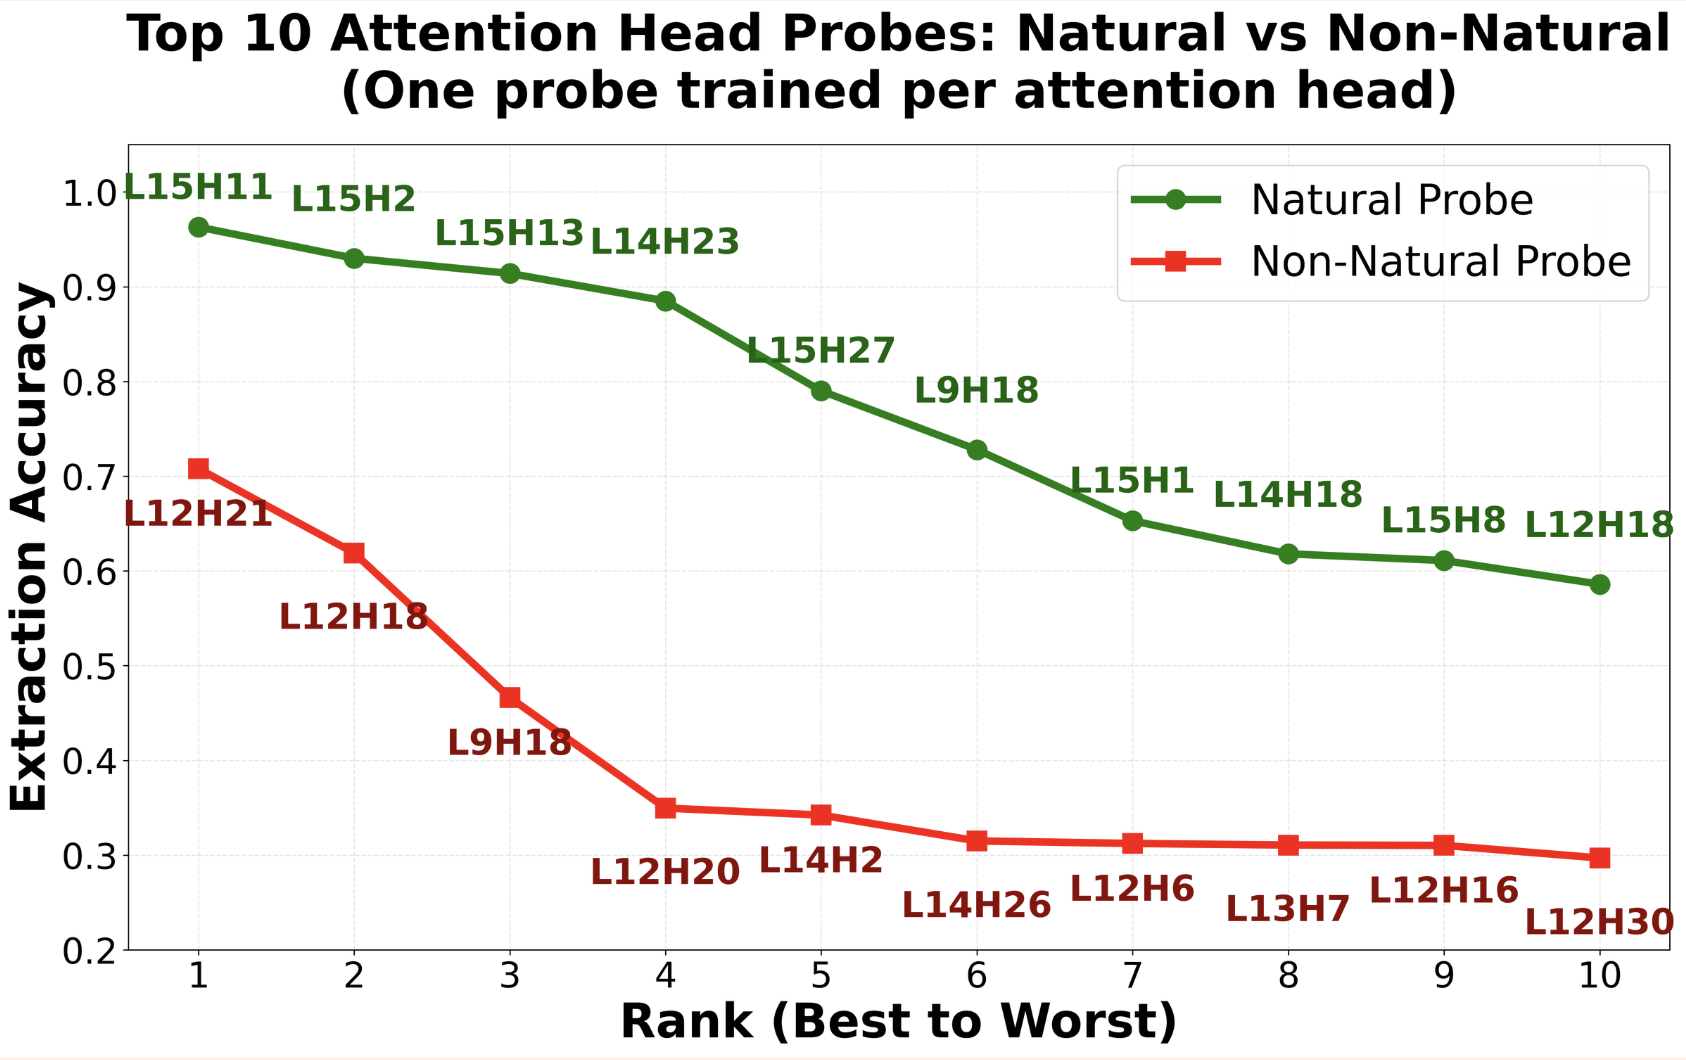
\includegraphics[width=\columnwidth]{natural_vs_non.png}
    \caption{Comparison of \textit{natural probe} (querying from the right) versus \textit{non-natural probe} (querying from the left) accuracy on the Favorite Color dataset. Each point represents the  probe accuracy for a given probe for a given head, ranked by accuracy of the probe. The natural probe consistently outperforms the non-natural probe, with the gap widening at higher ranks.}
    \label{fig:natural_vs_non}
    \end{figure}
\subsubsection{The Probe is Not Overly Powerful}
\label{sec:probe_not_strong}

If the probe were too expressive, it could achieve high accuracy on any head regardless of whether that head stores relevant information. However, \cref{tab:top_heads} shows that the \textit{natural probe} achieves high accuracy on only a small fraction of heads. The top head (L15H11) reaches 96.3\%, but accuracy drops sharply: by rank 5 it falls below 80\%, and by rank 10 below 60\%. Most of the 768 heads yield near-chance performance.


This concentration of high-accuracy probes in a small subset of heads, rather than diffuse success across all 768 heads, indicates that the probe is identifying genuine ``memory heads'' rather than exploiting spurious correlations.

\subsubsection{Querying from the Right Outperforms Querying from the Left}
\label{sec:natural_vs_nonnatural}

A core design choice in our probing approach is querying the state from the right, mirroring the model's native mechanism (\cref{eq:state_query}). To validate that this direction is not an arbitrary choice, we compare the \textit{natural probe} against a \textit{non-natural probe} that queries from the left (\cref{eq:probe_wrong}).

The \textit{natural probe} significantly outperforms the \textit{non-natural probe}: the best \textit{natural probe} reaches 96.3\%, while the best \textit{non-natural probe} achieves only 70.8\%.

This gap confirms that memory is encoded in a manner consistent with the model's native query mechanism (\cref{eq:state_query}). Probing from the right extracts information effectively; probing from the left does not. \cref{fig:natural_vs_non} visualizes this comparison across the top 10 heads for each probe type.


\subsection{Causal Effect of Memory Heads}
\label{sec:causal_results}

To verify that probe-identified heads play a causal role in storing memory, we perform counterfactual patching experiments on 50 sample pairs from the Favorite Color dataset. \cref{tab:causal} shows the results.

\begin{table}[t]
\centering
\small
\caption{Counterfactual patching results. ``Correct'': the model outputs the original property; ``Switched'': the model outputs the counterfactual property; ``Neither'': any other output.}
\label{tab:causal}
\begin{tabular}{@{}lccc@{}}
\toprule
Method & Correct & Switched & Neither \\
\midrule
Baseline & 90\% & 0\% & 10\% \\
Natural probe (top 0.5\%) & 14\% & 36\% & 50\% \\
Random (0.5\%) & 86\% & 2\% & 12\% \\
All heads & 0\% & 76\% & 24\% \\
\bottomrule
\end{tabular}
\end{table}

The results show a striking asymmetry. Patching just 4 heads out of 768 (the top 0.5\% by \textit{natural probe} accuracy) is enough to make the model switch to the counterfactual property 36\% of the time, a dramatic behavioral shift from a relatively small intervention. In contrast, patching the same number of randomly selected heads (averaged over 5 seeds) yields only a 2\% switch rate. This large gap confirms that the heads identified by the \textit{natural probe} are not merely correlated with memory storage but play a direct causal role in the model's retrieval process. Patching all 768 heads provides an upper bound of 76\%, indicating that these few probe-selected heads already account for a substantial fraction of the model's total memory capacity.

\subsection{The Bottleneck is Querying, Not Storage}
\label{sec:bottleneck}

A key observation emerges from comparing probe performance to model performance. While our probes extract the correct binding with up to 96.3\% accuracy, the model's own ability to answer questions about these bindings is substantially lower.

When we prompt the model using the template in \cref{fig:prompt_template}, its accuracy is far below probe accuracy. This gap implies that the information \emph{is stored} in the state (the probe finds it) but the model struggles to \emph{query} it effectively during generation.

This finding challenges the common assumption that SSMs' limitations stem from insufficient memory capacity \cite{jelassi2024repeat,yang2024deltanet,grazzi2024statetracking}. Instead, our results suggest that the bottleneck lies in the model's ability to formulate effective queries.

\subsection{Universal Memory Heads}
\label{sec:universal_heads}

We analyze whether the same heads are important across different semantic domains by comparing top-performing heads on the Favorite Color dataset versus Lives in City.

We find substantial overlap: 7 of the top 10 heads are shared across both datasets. \cref{fig:universal_heads} visualizes this overlap, showing that the majority of top-performing heads are consistent across semantically distinct tasks. This suggests the existence of \emph{universal memory heads} that specialize in entity-property binding regardless of semantic content. We defer investigation of the mechanism underlying these heads to future work.

\begin{figure}[t]
\centering
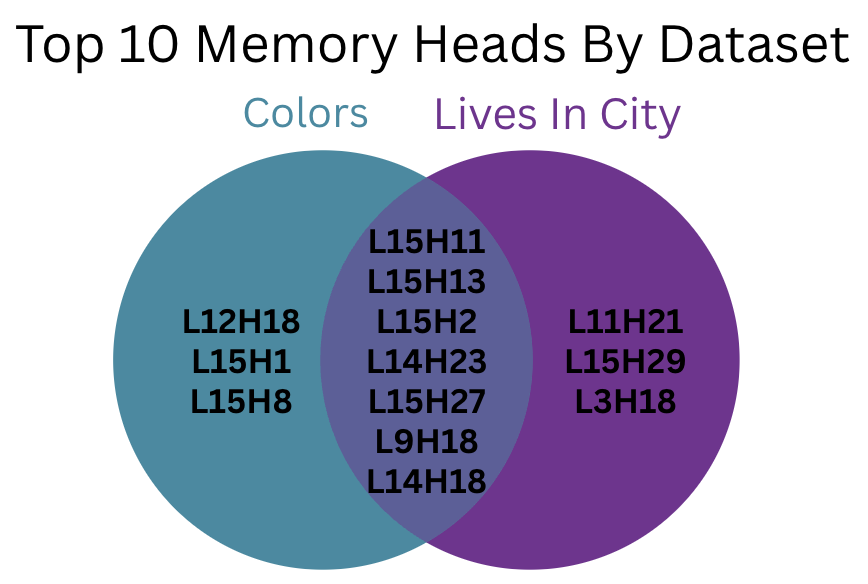
\includegraphics[width=0.8\columnwidth]{universal_heads.png}
\caption{Overlap of top 10 heads ranked by \textit{natural probe} accuracy across two different datasets. Seven heads (shown in the intersection) achieve high accuracy on both Favorite Color and Lives in City tasks, demonstrating domain-general memory storage capabilities.}
\label{fig:universal_heads}
\end{figure}

\subsection{Semantic Collision Accelerates Forgetting}
\label{sec:semantic_collision}

We investigate how context affects memory retention by measuring probe accuracy as a function of token distance from the information. We observe that increased semantic similarity between the prompt content and the target subject accelerates the model's forgetting rate, as can be seen in \cref{fig:compare_accuracy_top_3,fig:compare_top_1}. 
When subsequent sentences discuss similar entities, probe accuracy degrades faster than when the intervening content is semantically distinct.
More specifically, we create two types of datasets: a homogeneous dataset containing only sentences of one type (e.g., "Lady Gaga's favorite animal is Fox"), 
and a mixed dataset that combines sentences from two different domains (e.g., favorite animals and favorite colors) in a ratio where the target domain represents only a small fraction (roughly 1/30) of the total sentences.

We hypothesize that this effect arises from the difficulty of encoding semantically similar key-value pairs in a fixed-size state matrix: when consecutive entries share similar key vectors, they compete for the same subspace and overwrite each other more aggressively. This interference mechanism is a direct consequence of the state update rule (\cref{eq:state_update}). Understanding and mitigating this collision effect is an interesting avenue for future work.

\begin{figure}[t]
\centering
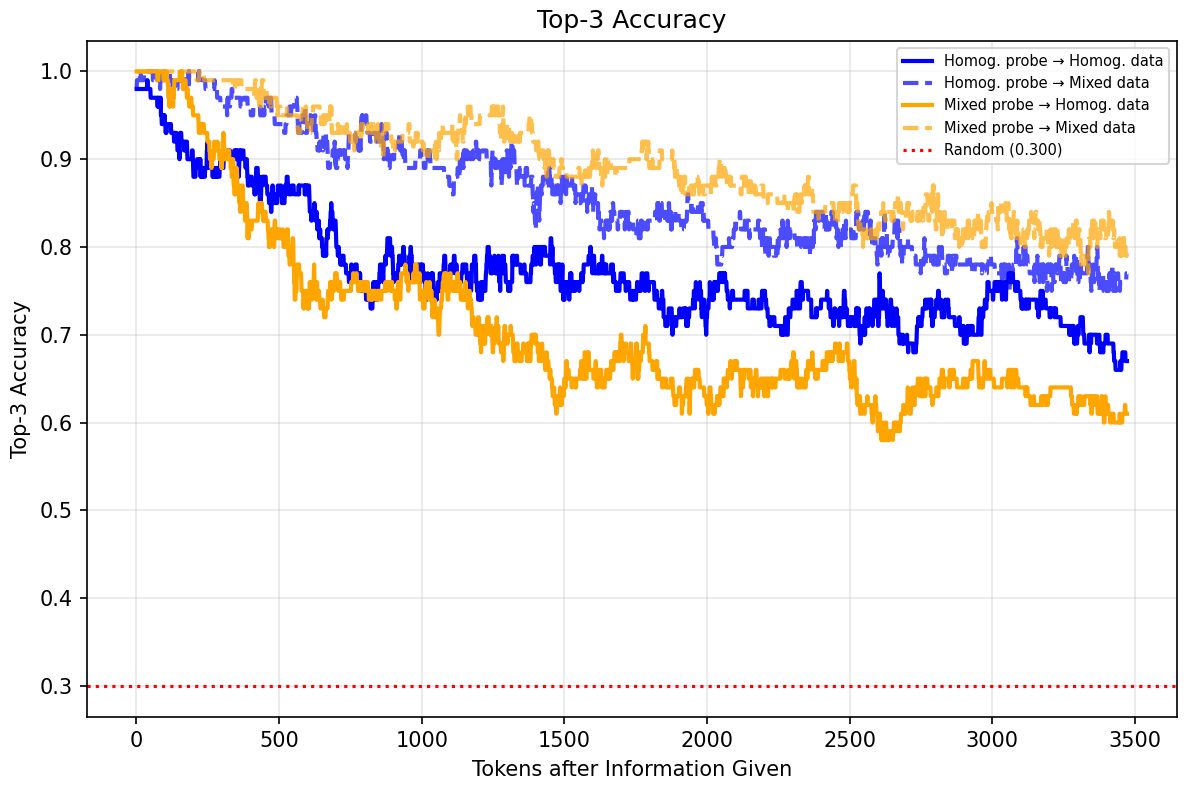
\includegraphics[width=\columnwidth]{compare_standalone_vs_combined_accuracy_top_3.png}
\caption{Top 3 accuracy of the homogeneous and mixed data probes on homogeneous and mixed data as a function of token distance from the binding pair we query.}
\label{fig:compare_accuracy_top_3}
\end{figure}


% =============================================================================
% Future Work
% =============================================================================
\section{Future Work}
\label{sec:future_work}

Our findings open several directions for future research.

A natural next step is to characterize the mechanism underlying universal memory heads. We have shown that a small subset of heads consistently stores entity-property bindings across semantically distinct domains, but the question of what makes these heads special remains open. Understanding their internal dynamics, whether they develop specialized decay patterns, allocate subspaces differently, or emerge from particular training dynamics, could inform architectural improvements and targeted fine-tuning strategies for sub-quadratic models.

\begin{figure}[t]
\centering
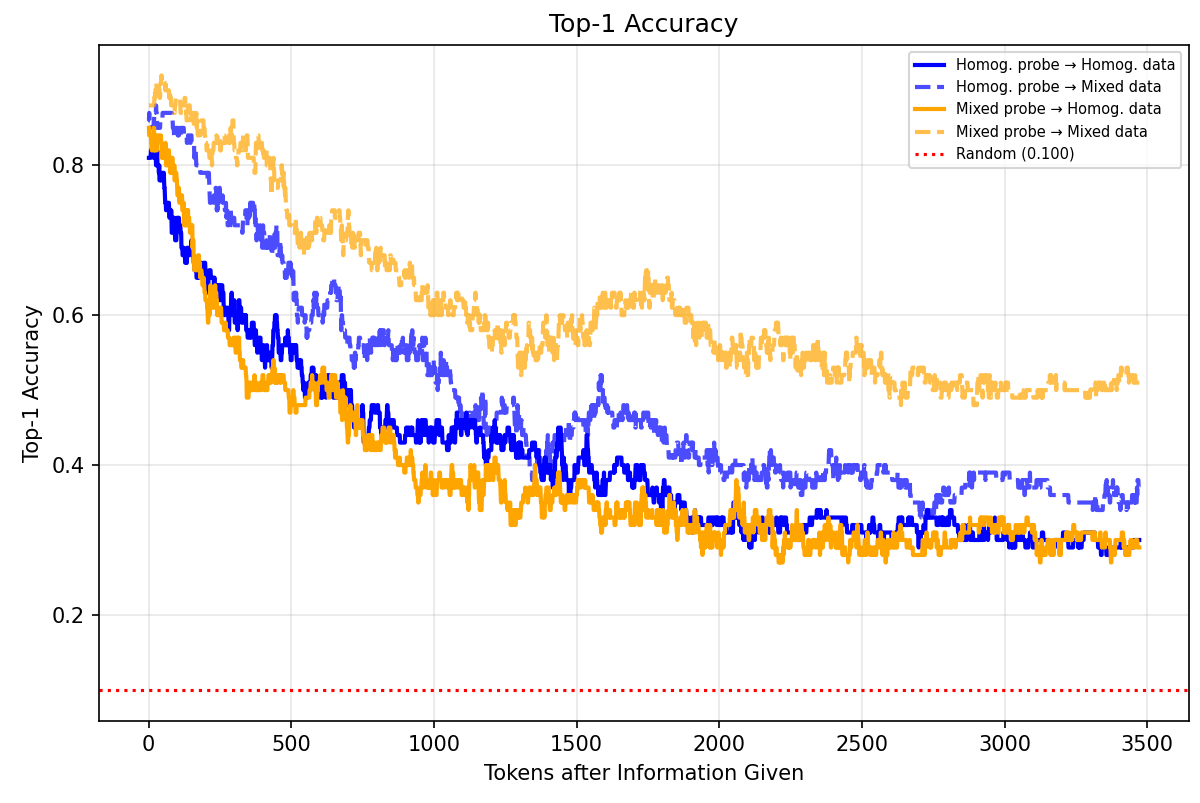
\includegraphics[width=\columnwidth]{compare_standalone_vs_combined_top_1.png}
\caption{Top 1 accuracy of the homogeneous and mixed data probes on homogeneous and mixed data as a function of token distance from the binding pair we query.}
\label{fig:compare_top_1}
\end{figure}


The gap between probe accuracy and model retrieval accuracy suggests that improving the query mechanism is a promising direction. Our probes demonstrate that the information is present in the state, yet the model fails to retrieve it reliably. Designing better query strategies, possibly inspired by the structure of successful probes, could improve SSM performance on tasks requiring in-context recall.

It would also be valuable to investigate how these findings scale. Our experiments focus on a 1.5B parameter model, and it remains to be seen whether larger SSMs exhibit the same concentration of memory in a few heads, whether more heads become memory-capable with scale, and whether the query bottleneck persists or diminishes.

Finally, the semantic collision phenomenon we observe opens a line of work on mitigating interference between similar entities. Exploring training objectives or architectural modifications that reduce subspace competition, such as encouraging orthogonal key representations for same-domain entities, could improve memory retention in settings where the context is semantically homogeneous.

% =============================================================================
% Limitations
% =============================================================================

% =============================================================================
% Conclusion
% =============================================================================
\section{Conclusion}
\label{sec:conclusion}

We investigated how state space models store and retrieve in-context information by probing their internal states. By designing probes that mirror the model's native right-multiplication query mechanism, we showed that entity-property bindings are reliably encoded in a small subset of heads, and that probing from the right substantially outperforms probing from the left. Counterfactual patching confirmed that these heads play a direct causal role in the model's outputs: replacing just 4 out of 768 heads is sufficient to alter the model's answer. Across semantically distinct domains, the same heads consistently emerge as the most informative, pointing to the existence of universal memory heads.

Perhaps most notably, probe accuracy far exceeds the model's own retrieval accuracy, indicating that the relevant information is present in the state but the model struggles to access it during generation. This suggests that the primary limitation of current SSMs lies not in storage capacity but in the effectiveness of the query mechanism. We also found that semantically similar context accelerates forgetting, likely due to subspace interference in the state matrix. Together, these findings point toward improving query strategies and reducing semantic collision as promising directions for closing the gap between what sub-quadratic models store and what they can retrieve.

\section{Limitations}
\label{sec:limitations}

Our study has several limitations. All experiments are conducted on a single model (RWKV-7 1.5B), so it remains unclear whether the findings generalize to other SSM architectures or to larger scales. The entity-binding datasets we use, while useful for controlled analysis, are synthetic and structurally simple compared to the kinds of factual associations that arise in natural text; it is possible that memory dynamics differ in more realistic settings. Additionally, several of our findings are observational rather than fully developed: we identify universal memory heads but do not explain the mechanism behind them, we show that the query bottleneck exists but do not propose a solution, and our hypothesis about semantic collision causing subspace interference is supported by indirect evidence but not formally tested. We view these as starting points for future investigation rather than definitive conclusions.

\section{AI Disclosure and Reflection}
\label{sec:ai_disclosure}

We used the Cursor IDE with several AI models throughout this project. On the code side, AI assisted with writing almost all of the code. On the writing side, AI helped draft and revise sections of this paper, with all content reviewed and edited by the authors.

% =============================================================================
% Bibliography
% =============================================================================
\bibliography{custom}

\end{document}
